\documentclass[12pt]{article}
\usepackage{enumerate}
\usepackage{notes}
\usepackage{oxford}

\begin{document}

\section{2017}

\subsection*{}  % 1
\begin{mdframed}
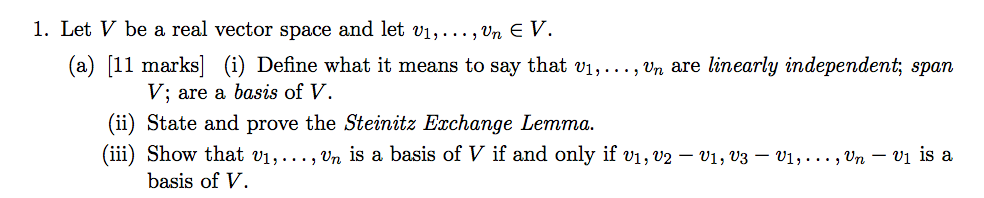
\includegraphics[width=400pt]{img/oxford-prelims-2017-A-1-1.png}
\end{mdframed}

\subsubsection*{(i)}
\begin{definition*}[Linear independence]
  Let $a_1, \ldots, a_n \in \R$. Then $v_1, v_2, \ldots, v_n$ are linearly
  independent if and only if the only solution to $\sum_{i=1}^n a_iv_i = 0$ is
  $a_1 = a_2 = \ldots = a_n = 0$.
\end{definition*}

\begin{definition*}[Span]
  $v_1, v_2, \ldots, v_n$ span $V$ if and only if for all $w \in V$ there exist
  $a_1, \ldots, a_n \in \R$ such that $\sum_{i=1}^n a_iv_i = w$.
\end{definition*}

\begin{definition*}[Basis]
  $v_1, v_2, \ldots, v_n$ are a basis for $V$ if and only if they span $V$ and
  they are linearly independent.
\end{definition*}


\newpage
\subsubsection*{(ii)}

\begin{claim*}
  $n+1$ vectors in $\R^n$ cannot be linearly independent.
\end{claim*}

\begin{proof}
  We want to show that there exists $\lambda_1, \ldots, \lambda_{n+1}$, not all
  zero, such that $\sum \lambda_ix_i = 0$.

  Suppose they are linearly independent. Then the first $n$ form a basis
  (assuming it is known that $n$ LI vectors span $\R^n$). Therefore the last
  one can be written as a linear combination of the first $n$.
\end{proof}

\begin{theorem*}[Steinitz Exchange Lemma]
  Let $V$ be a vector space. Let $v_1, \ldots, v_m$ be a linearly independent
  set of vectors in $V$, and let $w_1, \ldots, w_n$ span $V$. Then,
  \begin{enumerate}[label=\roman*)]
  \item $m \leq n$
  \item $v_1, \ldots, v_m, w_{m+1}, \ldots, w_n$ also spans $V$, possibly after
    reordering the $w_i$.
  \end{enumerate}
\end{theorem*}

[Informally: if a set of vectors is linearly independent, then it can be no
larger than a spanning set, and it can be made into a spanning set by
contributing vectors from an existing spanning set.]

\begin{proof}~\\
  Let $P(k)$ be the following proposition: the theorem is true for $m = 0, 1, \ldots, k$.

  Fix an arbitrary integer $k > 0$. We want to show that $P(k)$ is true.

  $P(0)$ is true, since the $w_i$ span $V$ by hypothesis.

  For induction, suppose $P(j)$ is true, where $j < k$. At this point, we know
  the following facts:~\\

  \begin{enumerate}[label=\roman*)]
  \item linearly independent vectors $v_1, \ldots, v_k$ exist, by hypothesis of $P(k)$
  \item $j < k$, by the induction hypothesis $P(j)$
  \item $j \leq n$, by the induction hypothesis $P(j)$
  \item $v_1, \ldots, v_j, w_{j+1}, \ldots, w_n$ spans $V$, by the induction hypothesis $P(j)$.
  \end{enumerate}
  ~\\
  (iv) implies that we can write $v_{j+1}$ as a unique linear combination:
  \begin{align*}
    v_{j+1} = \sum_{i=1}^j \lambda_iv_i + \sum_{i=j+1}^n\mu_iw_i.
  \end{align*}
  (i) and (ii) imply that $v_1, \ldots, v_{j+1}$ are linearly independent, and
  therefore that at least one of the $\mu_i$ is non-zero.








  % Let $P(m)$ be the following proposition: given linearly independent
  % $w_1, \ldots, w_m \in V$, then, possibly after reordering the $v_i$, the set
  % $\{w_1, \ldots, w_m, v_{m+1}, \ldots, v_n\}$ is a basis for $V$.

  % Note that the dimension of $V$ is $n$.

  % $P(n)$ is true, since the $w_i$ are linearly independent by definition and
  % every set of $n$ linearly independent vectors in $V$ spans $V$.

  % Suppose for induction that $P(k)$ is true. So we have that
  % $w_1, \ldots, w_k, v_{k+1}, \ldots, v_n$ is a basis. We want to show that
  % $P(k-1)$ is true.

  % Consider $w_1, \ldots, w_{k-1}$. These span a subspace $U \subset V$ of
  % dimension $k-1$.

  % We have $k$ unused vectors $v_1, \ldots, v_k$. Since these are linearly
  % independent, at least one of them must not be in $U$. Reorder them so that
  % $v_k \notin U$. Then $w_1, \ldots, w_{k-1}, v_k, v_{k+1}, \ldots, v_n$ are a
  % linearly independent set of size $n$, and therefore span $V$, so $P(k-1)$ is
  % true.


\end{proof}

\newpage
\subsubsection*{(iii)}

$\implies$\\


$\impliedby$\\
Let $v_1, v_2 - v_1, \ldots, v_n - v_1$ be a basis of $V$.

Then for all $w \in V$ there exist $a_1, \ldots, a_n$, all non-zero, such that
\begin{align*}
  a_1v_1 + \sum_{i=2}^n a_i(v_i - v_1) = w.
\end{align*}
Therefore
\begin{align*}
  \Big(a_1 - \sum_{i=2}^na_i\Big)v_1 + \sum_{i=2}^n a_iv_i = w.
\end{align*}

So $v_1, v_2, \ldots, v_n$ span $V$ (TODO: but how do we know that $a_1 \neq \sum_{i=2}^na_i$?)

TODO: linear independence

~\\
\newpage
\begin{mdframed}
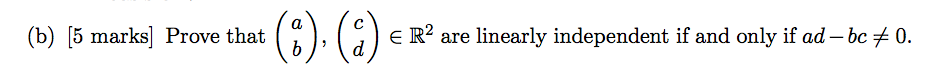
\includegraphics[width=400pt]{img/oxford-prelims-2017-A-1-2.png}
\end{mdframed}

\renewcommand{\cvec}[2]{\begin{pmatrix}#1\\#2\end{pmatrix}}

Let $x_1 = \cvec{a}{b}$ and $x_2 = \cvec{c}{d}$

We prove the negation; that $x_1, x_2$ linearly dependent is equivalent to
$ad - bc = 0$.

First, we prove that $x_1, x_2$ linearly dependent implies $ad - bc = 0$.

Since they are linearly dependent, there exists $\lambda_1, \lambda_2 \in \R$
such that $\lambda_1x_1 + \lambda_2x_2 = 0$, with at least one of
$\lambda_1, \lambda_2$ non-zero.

Suppose, without loss of generality, that $\lambda_1 = 0$. Then
$\lambda_2 \neq 0$ and therefore $c = d = 0$, and therefore $ad - bc = 0$.

The remaining case is that $\lambda_1 \neq 0$ and $\lambda_2 \neq 0$. Then
\begin{align*}
  \begin{cases}
    a\lambda_1 + c\lambda_2 = 0\\
    b\lambda_1 + d\lambda_2 = 0,
  \end{cases}
\end{align*}
therefore
\begin{align*}
\lambda_1 &= -\frac{c}{a}\lambda_2,
\end{align*}
therefore
\begin{align*}
  \Big(-\frac{bc}{a} + d\Big)\lambda_2 = 0,
\end{align*}
therefore
\begin{align*}
  ad - bc = 0.
\end{align*}
~\\
\newpage
\begin{mdframed}
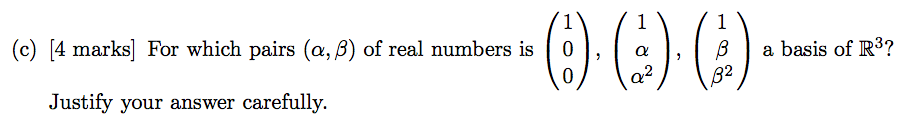
\includegraphics[width=400pt]{img/oxford-prelims-2017-A-1-3.png}
\end{mdframed}

~\\
\subsection*{}  % 2
\begin{mdframed}
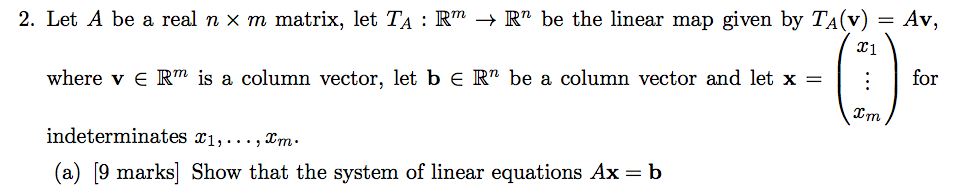
\includegraphics[width=400pt]{img/oxford-prelims-2017-A-2-1.png}
\end{mdframed}

\subsection*{}  % 2.a.i
\begin{mdframed}

\includegraphics[width=400pt]{img/oxford-prelims-2017-A-2-1-1.png}
\end{mdframed}

By definition,  $\Im T_A = \{Ax: x \in \R^m\}$.

Let $S$ denote the proposition ``$Ax = b$ has a solution''.

By the definition of ``has a solution'', $S$ is equivalent to the proposition
``there exists $x \in \R^m$ such that $Ax = b$''.

We see that $S \implies b \in \Im T_A$, and also that $b \in \Im T_A \implies S$.

% By definition, $\Im T_A = \{b : \exists x : Ax = b\}$, we then have $b \in \Im
% T_A$. Therefore $S \implies b \in \Im T_A$.

% Conversely if $b \in \Im T_A$ then

% ``$Ax = b$ has a solution'' is logically equivalent to ``$b \in \Im T_A$'' by
% the definitions of ``have a solution'' and $\Im$: they both mean ``there exists
% $x \in \R^m$ such that $Ax = b$''.

% The meaning of ``$Ax = b$ has a solution'' is: there exists $x \in \R^m$ such that
% $Ax = b$.

% If $b \in \Im T_A$ then, by definition of $\Im$, $Ax = b$ has a solution.

% Conversely, if $Ax = b$ has a solution, then $b \in \Im T_A$.

\subsubsection*{} % 2.a.ii
\begin{mdframed}
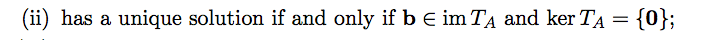
\includegraphics[width=400pt]{img/oxford-prelims-2017-A-2-1-2.png}
\end{mdframed}

Let $S_u$ denote the proposition ``$Ax = b$ has a unique solution''.

\begin{claim*}
  $S_u \implies \Big(b \in \Im T_A ~~\text{and}~~ \ker T_A = \{0\}\Big)$.
\end{claim*}

\begin{proof}
Firstly, since $S_u \implies S$, we know from part (i) that
$S_u \implies b \in \Im T_A$.

Suppose $S_u$ is true and let $x$ be the unique solution.

We know that $0 \in \ker A$ since $A(0) = A(x - x) = Ax - Ax = 0$ by the
linearity of $A$.

Now suppose there exists $y \neq 0 \in \ker T_A$. But
\begin{align*}
A(x + y) = Ax + Ay = b + 0 = b,
\end{align*}
so $x + y \neq x$ is also a solution; a contradiction. Therefore no such $y$
exists and we see that $S_u \implies \ker T_A = \{0\}$.
\end{proof}

\begin{claim*}
  $\Big(b \in \Im T_A ~~\text{and}~~ \ker T_A = \{0\}\Big) \implies S_u$.
\end{claim*}

\begin{proof}
  Suppose $b \in \Im T_A$. Then we know from part (i) that $S$ is true. So let
  $x$ be a solution.

Now suppose that $\ker T_A = \{0\}$ and that $y \neq x$ is another solution. But then
\begin{align*}
  A(x - y) = Ax - Ay = b - b = 0,
\end{align*}
so $x - y \neq 0 \in \ker T_A$; a contradition. Therefore if $\ker T_A = \{0\}$
then no such $y$ exists.
\end{proof}

\subsubsection*{} % 2.a.iii
\begin{mdframed}
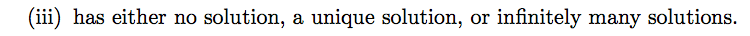
\includegraphics[width=400pt]{img/oxford-prelims-2017-A-2-1-3.png}
\end{mdframed}

Suppose $Ax = b$ has $n > 1$ solutions and let the first two such solutions be
$x_1$ and $x_2$. Then there are uncountably infinitely many solutions, since
for all $\alpha \in \R$
\begin{align*}
A\Big(x_1 + \alpha (x_2 - x_1)\Big) = Ax_1 + \alpha(Ax_2 - Ax_1) = b + \alpha(b - b) = b.
\end{align*}

~\\
\subsection*{} % 2.b
\begin{mdframed}
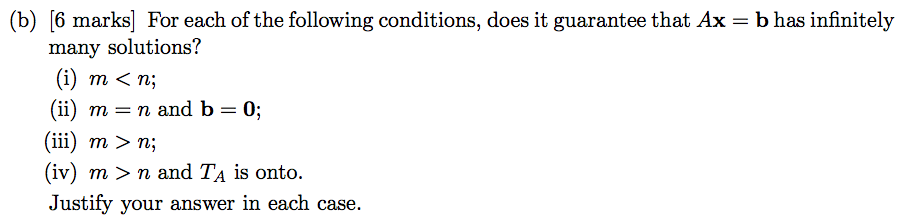
\includegraphics[width=400pt]{img/oxford-prelims-2017-A-2-2.png}
\end{mdframed}

\subsubsection*{(i)} The mapping takes vectors in a lower dimensional space and
outputs vectors in a higher dimensional space. E.g. suppose $T_A:\R^1 \to \R^2$
and let $A = \scvec{s}{t}$. Then $Ax = (xs, xt)$ i.e. $\Im T_A$ is a line
through the origin.

\begin{align*}
  m &=    \dim(\ker T_A) + \dim(\im T_A)\\
    &\leq \dim(\ker T_A) + n\\
\end{align*}
~\\
\subsection*{} % 2.c
\begin{mdframed}
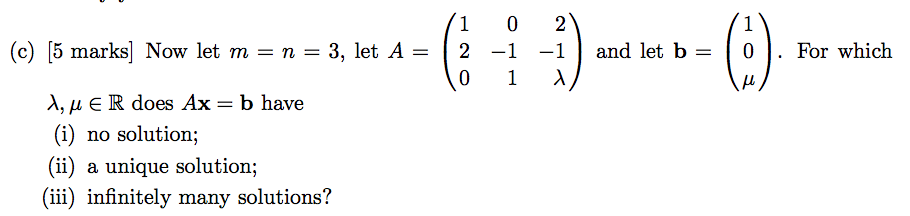
\includegraphics[width=400pt]{img/oxford-prelims-2017-A-2-3.png}
\end{mdframed}

\end{document}
